\subsection*{Ziel 1: Literaturrecherche}

\subsubsection{Frage 1.1: Technologien Synthetische Daten}
\begin{description}[style=nextline, font=\bfseries\sffamily]
    \item[Methodik] 
        Für die initiale Literaturrecherche wurde der folgende Suchstring für die Datenbanken IEEEXplore und PubMed verwendet:
            \begin{quote}
            ((\enquote{synthetic data generation} OR \enquote{synthetic clinical data} OR \enquote{synthetic data} OR \enquote{synthetic patient} OR \enquote{synthetic patient data} OR \enquote{synthetic EHR} OR \enquote{Synthea}) \textbf{AND} (\enquote{large language models} OR \enquote{LLM} OR \enquote{generative AI} OR \enquote{autonomous agents} OR \enquote{agent-based} OR \enquote{machine learning}) \textbf{AND} (\enquote{clinical workflows} OR \enquote{patient history} OR \enquote{medical records} OR \enquote{case vignettes} OR \enquote{longitudinal} OR \enquote{simulated patients}))
            \end{quote}

        Für die Auswahl der Publikationen wurden die folgenden Ein- und Ausschlusskriterien definiert:
    \begin{itemize}
        \item \textbf{Einschlusskriterien:}
        \begin{itemize}
            \item Generierung von synthethischen Patientenaten durch Sprachmodelle oder nicht-Sprachmodell-basierte Agenten
        \end{itemize}
        \item \textbf{Ausschlusskriterien:}
        \begin{itemize}
            \item Generierung von Daten die nicht im Kontext der Medizin stehen
            \item Die Methode zur Generierung der Daten wird nicht genannt.
        \end{itemize}
    \end{itemize}
        Mit den resultierenden Publikationen wurden ein Titel-, Abstract- und Volltext-Screening durchgeführt
    \nopagebreak 
    \begin{center}
        \begin{minipage}{\linewidth}
            \centering
            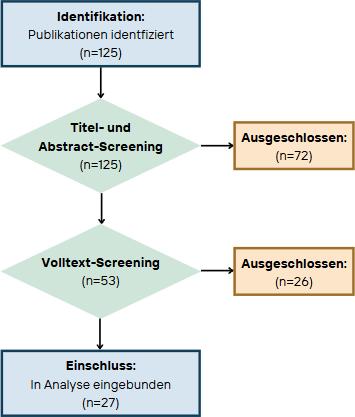
\includegraphics[width=0.5\textwidth]{Artikel/pictures/SynDatenFlowchart.png}
            \captionof{figure}{Flussdiagramm des Auswahlprozesses der Paper für die Literaturrecherche zur Generierung von synthetischen Patientendaten.} 
            \label{fig:syn_flow_chart}
        \end{minipage}
    \end{center}

    \item[Ergebnisse]

        Die Analyse der identifizierten Quellen ($n = 27$) erfolgte in zwei Schritten: Zunächst eine Klassifizierung der Artikeltypen und anschließend eine technische Differenzierung der darin beschriebenen Methoden.
    \item[Verteilung der Artikeltypen]
        Die Verteilung der Artikeltypen gliedert sich in zwei Kernbereiche: Reviews und methodische Benchmarks (n=10) dienten primär der Identifikation des aktuellen Stands der Technik sowie dem Vergleich bestehender Frameworks. Den komplementären Teil bildet die Primärliteratur zu spezifischen Methoden (n=17), welche konkrete Implementierungen oder neu entwickelte Algorithmen beschreibt.
    \item[Eingesetzte Technologien] 
        Zur Abbildung der technologischen Breite wurden die Ansätze wie folgt kategorisiert:
        
        \begin{itemize}[leftmargin=1.5em, labelsep=0.5em, itemsep=4pt, topsep=4pt]
            \item \textbf{LLMs \& Transformer} ($n = 9$): 
            Fokus auf die Generierung synthetischer Patientenakten durch Sprachmodelle.
            
            \item \textbf{Generative Adversarial Networks (GANs)} ($n = 4$): 
            Einsatz primär für tabellarische Daten und Bilddaten.
            
            \item \textbf{Agenten-basierte Simulation (Synthea)} ($n = 2$): 
            Regelbasierte Erzeugung lebenslanger Patientenhistorien.
            
            \item \textbf{Diffusion \& Interaktive Frameworks} ($n = 2$): 
            Neuere Ansätze zur probabilistischen Datenerzeugung.
        \end{itemize}
    \item[Beantwortung]
        Die technologische Landschaft wird primär durch den Einsatz von Large Language Models (LLMs) und Generative Adversarial Networks (GANs) geprägt, ergänzt durch regelbasierte Systeme wie das Synthea-Framework.
\end{description}

\subsubsection{Frage 1.2: Technologien Einbindung Sensor Daten}
\begin{description}[style=nextline, font=\bfseries]

    \item[Methodik] 
    Die methodische Grundlage dieser Arbeit bildet eine systematische Literaturrecherche in den Datenbanken PubMed und IEEE Xplore (Stand: März 2026). 
    
    Für die Recherche in PubMed wurde folgende Suchstrategie (Search String) verwendet:
    
    \begin{quote}
    ((\enquote{Hospital Information Systems}[MeSH] OR \enquote{Electronic Health Records}[MeSH]) 
    AND (\enquote{sensor\textasteriskcentered} OR \enquote{sensor data} OR \enquote{wearable\textasteriskcentered}) 
    AND (\enquote{storage} OR \enquote{archiving} OR \enquote{persistence} OR \enquote{NoSQL} OR \enquote{SQL} OR \enquote{Time-series database} OR \enquote{openEHR} OR \enquote{FHIR} OR \enquote{repository})) 
    NOT (\enquote{Blockchain} OR \enquote{Security} OR \enquote{Cryptography} OR \enquote{Privacy Preservation} OR \enquote{Cybersecurity}))
    \end{quote}
    
    Für die Recherche in IEEE Xplore wurde folgender Search String angewendet:
    
    \begin{quote}
    ((\enquote{Hospital Information System\textasteriskcentered} OR \enquote{Electronic Record\textasteriskcentered}) 
    AND (\enquote{sensor\textasteriskcentered} OR \enquote{sensor data} OR \enquote{wearable\textasteriskcentered}) 
    AND (\enquote{storage} OR \enquote{archiving} OR \enquote{persistence} OR \enquote{NoSQL} OR \enquote{SQL} OR \enquote{Time-series database} OR \enquote{openEHR} OR \enquote{FHIR} OR \enquote{repository})) 
    NOT (\enquote{Blockchain} OR \enquote{Security} OR \enquote{Cryptography} OR \enquote{Privacy Preservation} OR \enquote{Cybersecurity}))
    \end{quote}
    
    Für die Auswahl der Primärliteratur wurden die folgenden Ein- und Ausschlusskriterien definiert:
    \begin{itemize}
        \item \textbf{Einschlusskriterien:}
        \begin{itemize}
            \item Nutzung von Sensordaten und deren explizite Integration in ein KIS oder eine elektronische Patientenakte (Electronic Health Record, EHR).
        \end{itemize}
        \item \textbf{Ausschlusskriterien:}
        \begin{itemize}
            \item Publikationen, die sich ausschließlich mit Datensicherheit, Datenschutz oder Kryptographie befassen.
            \item Arbeiten, die lediglich die Erhebung von Sensordaten beschreiben, ohne eine Integration in ein KIS/EHR vorzusehen.
            \item Beiträge mit einem reinen Fokus auf Machine-Learning-Algorithmen (ohne systemarchitektonischen Bezug).
        \end{itemize}
    \end{itemize}
    
    \nopagebreak 
    \begin{center}
        \begin{minipage}{\linewidth}
            \centering
            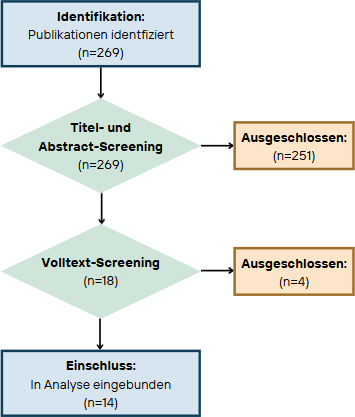
\includegraphics[width=0.5\textwidth]{pictures/SensorDatenFlowchart.png}
            \captionof{figure}{Flussdiagramm des Auswahlprozesses der Paper für die Literaturrecherche zur Integration der Sensordaten.} 
            \label{fig:sensor_flow_chart}
        \end{minipage}
    \end{center}
    \vspace{1ex}

    Die Literatursuche und das anschließende Screening führten zu folgenden Ergebnissen:
    
    In PubMed wurden initial 69 Ergebnisse identifiziert. Nach einem Titel- und Abstract-Screening wurden 10 Publikationen als relevant eingestuft. Das anschließende Volltext-Screening führte zum Ausschluss von zwei weiteren Arbeiten, sodass insgesamt 8 Publikationen aus PubMed in die Analyse einbezogen wurden.
    
    In IEEE Xplore wurden initial 200 Ergebnisse gefunden. Nach dem Titel- und Abstract-Screening verblieben 8 relevante Treffer. Im Zuge des Volltext-Screenings wurden ebenfalls zwei Arbeiten ausgeschlossen, woraus sich 6 finale Publikationen aus IEEE Xplore für die Synthese ergaben.
    
    Die insgesamt $n = 14$ identifizierten Quellen wurden quantitativ analysiert und manuell hinsichtlich der verwendeten Schnittstellenstandards kategorisiert. Der kombinierte Ablauf der Literaturrecherche in PubMed und IEEE Xplore ist im Flussdiagramm in Abbildung \ref{fig:sensor_flow_chart} dargestellt.

    \item[Ergebnisse] 
    Die Analyse zeigt eine deutliche Dominanz des HL7 FHIR Standards, der in $n = 11$ Artikeln Anwendung findet. Lediglich $n = 3$ Quellen setzen auf klassische REST-Schnittstellen zur Datenübertragung.

    \item[Beantwortung] 
    Der Dateneinzug erfolgt primär über den HL7 FHIR Standard oder einfache REST-Schnittstellen. Bemerkenswert ist, dass keine der untersuchten Arbeiten ein kontinuierliches Daten-Streaming in das KIS beschreibt; stattdessen erfolgt die Integration ausschließlich im Batch-Processing-Verfahren durch gezieltes Pulling von den Servern.

\end{description}

\subsubsection{Frage 1.3: Anforderungen an Synthetische Daten}
\begin{description}[style=nextline, font=\bfseries]

    \item[Methodik] 
    Die methodische Grundlage bildet eine systematische Literaturrecherche in den Datenbanken PubMed und IEEE Xplore (Stand: März 2026). Aus den identifizierten Quellen wurden die von den Autoren explizit formulierten Anforderungen manuell extrahiert, um eine ungefilterte Vergleichsbasis für die weiteren Analysen zu schaffen.

    \item[Ergebnisse] 
    Aus den Papern ergaben sich die folgenden Anforderugen:
    \begin{itemize}[leftmargin=1.5em, labelsep=0.5em, itemsep=4pt, topsep=4pt]
    \item \textbf{Statistische Fidelität:} Synthetische Daten müssen die statistischen Eigenschaften des Originaldatensatzes präzise replizieren, insbesondere die Randverteilungen der Variablen und komplexe Korrelationsstrukturen. Hochdimensionale Krankheitskodes sollten dabei eine Korrelation der Kodewahrscheinlichkeiten von R2>0,9 erreichen. \citep{chen_generating_2025} \citep{theodorou_synthesize_2023}
    
    \item \textbf{Strukturelle Integrität:} Es wird eine hierarchische Konsistenz über multiple Tabellen hinweg gefordert (z. B. zwischen Patientenstammdaten und Laborwerten). Zudem müssen klinisch bedeutsame Fehlwerte (Informative Missingness) explizit modelliert werden.\citep{josling_novel_2026}
    
    \item \textbf{Temporale Dynamik:} Bei longitudinalen Daten müssen sowohl die sequenziellen Abhängigkeiten klinischer Ereignisse als auch die spezifischen Zeitintervalle (Inter-visit Gaps) realistisch abgebildet werden. \citep{josling_novel_2026} \citep{theodorou_synthesize_2023}
    
    \item \textbf{Klinische Nutzbarkeit (Utility):} Die Daten müssen im "Train-Synthetic-Test-Real" (TSTR) Framework validiert werden, um sicherzustellen, dass auf synthetischen Daten trainierte Modelle auf realen Daten performant sind. In spezialisierten Domänen wie der Kardiologie wird zudem eine klinische Kohärenz und medizinische Relevanz gefordert, die durch Fachexperten validiert wurde. \citep{theodorou_synthesize_2023} \citep{jung_clinical_2025}
    
    \item \textbf{Datenschutz und Sicherheit:} Eine zentrale Anforderung ist die Vermeidung von Overfitting, um Re-Identifizierungsrisiken zu minimieren. Hierfür wird oft die Integration von Differential Privacy (DP) und die Messung der $\epsilon$-Identifizierbarkeit gefordert. \citep{tsao_health_2023} \citep{hahn_contribution_2022} \citep{chen_generating_2025}
    
    \item \textbf{Governance und Ethik:} Die Generierung sollte den FAIR-Prinzipien (Findable, Accessible, Interoperable, Reusable) entsprechen. Bei der Verwendung von Daten marginalisierter Gruppen müssen zudem die CARE-Prinzipien (Collective benefit, Authority to control, Responsibility, Ethics) beachtet werden. \citep{tsao_health_2023}
    
    \item \textbf{Bias-Vermeidung:} Die Generierungsprozesse dürfen bestehende algorithmische Biases aus den Originaldaten nicht verstärken oder perpetuieren. \citep{theodorou_synthesize_2023}
    \end{itemize}

    \item[Beantwortung] 
    Zusammenfassend lassen sich die in der Literatur formulierten Anforderungen in sieben Kernbereiche unterteilen: statistische Fidelität, strukturelle Integrität, temporale Dynamik, klinische Nutzbarkeit, Datenschutz, Governance/Ethik sowie die aktive Bias-Vermeidung.

\end{description}

% --- ZIEL 2 ---
\subsection*{Ziel 2: Definition der Qualitätskriterien}

\subsubsection{Frage 2.1: Befragung von Expert*innen}

\begin{description}[style=nextline, font=\bfseries]

    \item[Methodik] 
    Zur Erhebung der Expertenanforderungen wurde im ersten Schritt ein strukturierter Gesprächsleitfaden konzipiert. Dieser diente als methodische Grundlage für die anschließenden Experteninterviews und fokussierte sich gezielt auf die medizinische, informationstechnische sowie didaktische Qualität der synthetisch generierten Patientendaten und der in das Lehre-KIS importierten Sensordaten. 

    Dies sind alle Fragen des Leitfadens: 
    \href{https://github.com/robinhefner/Research-Project/blob/5359f58b92f2480c59e9677c2e41ec0f7c742b21/Gespr%C3%A4chsleitfaden_Qualit%C3%A4tskriterien.pdf}{Leitfaden Qualitätskriterien}
    \\

    \vspace{1em}
    Im Anschluss an die Ausarbeitung des Leitfadens erfolgte die Durchführung der eigentlichen Experteninterviews. Hierbei wurde ein zielgruppenadaptierter Ansatz gewählt, um die Befragung optimal an die jeweilige Fachexpertise der Interviewpartner anzupassen. Dies bedeutet konkret, dass nicht jedem Experten der vollständige Fragenkatalog vorgelegt wurde: Personen mit primär medizinischem Hintergrund wurden nicht zu informationstechnischen Details befragt, ebenso wie technische Experten von den spezifisch medizinischen Qualitätskriterien ausgenommen waren.

    \item[Ergebnisse] 
    Durch den gewählten Ansatz konnten insgesamt sechs qualitative Interviews erfolgreich realisiert werden. Die Kohorte der Befragten setzte sich aus drei Personen mit medizinischem Hintergrund sowie drei Person mit informationstechnischer Spezialisierung zusammen. Ein essenzielles Auswahlkriterium, das fünf Experten erfüllten, war ihre ausgewiesene praktische Erfahrung im Bereich der akademischen Lehre. Die Befragung lieferte umfassende, protokollierte Datenbasen für die anschließende Auswertung.

    \item[Beantwortung] 
    Die Befragung der Expert*innen wurde erfolgreich über sechs qualitative, zielgruppenadaptierte Interviews auf Basis eines dreigeteilten Leitfadens (Medizin, IT, Didaktik) durchgeführt. Dadurch konnte ein breites, interdisziplinäres Spektrum an praktischer Lehrerfahrung für die nachfolgende Kriterienauswertung erfasst werden.

\end{description}

\subsubsection{Frage 2.2: Analyse der Ergebnisse: Welche Anforderungen haben Spezialisten an die Daten?}

\begin{description}[style=nextline, font=\bfseries]

    \item[Methodik] 
    Die methodische Auswertung der erhobenen Daten erfolgte über eine qualitative Analyse der zuvor angefertigten Interviewprotokolle. Ziel dieser Analyse war es, die Aussagen der Experten systematisch zu strukturieren, Gemeinsamkeiten zu identifizieren und daraus die übergeordneten Kernanforderungen an die Datenqualität abzuleiten.

    \item[Ergebnisse] 
    Die qualitative Analyse der Interviewprotokolle führte zur Identifikation von vier primären Hauptkriterien für die Datenqualität:
    \begin{enumerate}
        \item \textbf{Klinische Plausibilität:} Beschreibt das medizinisch logische Zusammenspiel von Symptomen, Diagnosen und Behandlungen. Das Spektrum reicht dabei von fehlerfreien Standardtherapien bis zu plausiblen Fehlbehandlungen.
        \item \textbf{Longitudinale Konsistenz:} Bezieht sich auf den langfristigen, korrekten Krankheitsverlauf über größere Zeiträume hinweg. Chronische Erkrankungen und Folgeuntersuchungen müssen lückenlos aufeinander aufbauen und dürfen keine unlogischen Sprünge aufweisen.
        \item \textbf{Zeitlich logische Abfolge:} Umfasst die korrekte Reihenfolge sowie die Realitätsnähe der zeitlichen Abstände einzelner klinischer Ereignisse (z.\,B. die Zeitspanne von der Erstdiagnose über die Intervention bis zur Nachsorge).
        \item \textbf{Gesamteindruck:} Aggregiert die vorgenannten Aspekte zu einem globalen Qualitätseindruck der Patientenakte, welcher maßgeblich die Akzeptanz und den didaktischen Nutzwert für die Studierenden bestimmt.
    \end{enumerate}

    \item[Beantwortung] 
    Die Spezialisten stellen insgesamt vier zentrale Anforderungen an die synthetischen Patientendaten: klinische Plausibilität, longitudinale Konsistenz, eine zeitlich logische Abfolge sowie einen stimmigen Gesamteindruck. Diese extrahierten Kernkriterien definieren die qualitativen Mindestanforderungen, die für eine erfolgreiche und akzeptierte Nutzung in der akademischen Lehre erfüllt sein müssen.

\end{description}

% --- ZIEL 3 ---
\subsection*{Ziel 3: Prototypische Implementierung}
\subsubsection{Frage 3.1: Generierung mittels Synthea}
\begin{description}[style=nextline, font=\bfseries]

    \item[Methodik] 
    Die Patientengenerierung erfolgte auf Basis des öffentlichen Synthea-Repositorys unter Einbeziehung der offiziellen Wiki-Dokumentation zur Modellierung klinischer Abläufe.

    \item[Hürden] 
    Im Implementierungsprozess wurden drei zentrale Herausforderungen adressiert: 
    \begin{itemize}[leftmargin=1.5em, labelsep=0.5em, itemsep=4pt, topsep=4pt]
        \item \textbf{Herkunft der Patienten:}
        Synthea generiert standadtmäßig Patienten die in den USA verortet sind. Das bedeutet im amerikanischen Gesundheitssystem behandelt werden und amerikanische Namen und Adressen besitzen. Die Lösung war es das Repository zu forken (Ein Fork ist eine Kopie eines Repositories, welches den selben Code und Sichtbarkeit besitzt wie das ursprüngliche Repository) und die EU/DE Properties, die von Synthea zur Verfügung gestellt werden zu nutzen und eigene Änderungen einzuführen um Patienten die in der EU / Deutschland verortet werden zu erhalten.
        Durch die zur Verfügung gestellten Properties von Synthea wurden Krankenhäuser, sowie Städte und Krankenkassen aus deutschland importiert. Die Änderungen die nachträglich noch erstellt wurden waren die Einführung deutscher Vor und Nachnamen, sowie deutscher Straßennamen, welche in Synthea auch synthetisch generiert werden.
        \item \textbf{Vorgenerierung einer kompletten Patientenhistorie:}
        Synthea erstellt für einen Patienten immer eine komplette lückenlose Patientnehistorie. Das bedeutet, dass von Geburt bis ggf. Tod die Geschichte eines Patienten erstellt wird. Für eine möglichst realistisches KIS ist dies jedoch wenig repräsentativ. Als Lösung haben wir hierfür die FHIR Bundle, die von Synthea erstellt werden in einzelne Transaktionen aufgeteilt. Hierdurch kann die Patientenhistorie aufgeteilt werden und nur bis zu einem bestimmten Punkt ins KIS importiert werden. Wie dies gestaltet werden soll, also bis zu welchem Punkt die Daten importiert werden und wo der Cut-Off gesetzt wird steht noch offen.
        \item \textbf{Ärzte in Synthea und der Umgang im KIS:}
        Synthea erstellt für einen Patienten immer eine Liste an Ärzten, die diesen über den Verlauf behandelt haben. Dies würde für das studiKIS bedeuten, das sich die Menge der Ärzte exponentiell erhöhen würde, da jeder Patient eine Vielzahl an Ärzten hat die ihn im Verlauf behandeln. Ein Lösungsansatz wird in den Ergebnissen zu Frage 3.c dargestellt.
    \end{itemize}

    \item[Ergebnisse] 
    Es wurde ein funktionsfähiger Workflow etabliert, der die bedarfsgerechte Erzeugung beliebig großer Patientenkollektive im standardisierten FHIR-Format ermöglicht.

    \item[Beantwortung] 
    Durch die gezielte Anpassung des Synthea-Frameworks und die Implementierung regionaler Spezifika konnte eine Pipeline geschaffen werden, die lokalisierte und prozessual steuerbare synthetische Patientendaten für die Systemintegration bereitstellt.

\end{description}

\subsubsection{Frage 3.2: Generierung mittels LLM} 
\textbf{Methodik:} Entwicklung eines Prompts, der es ermöglicht strukturierte klinische Daten als FHIR Bundle zu erzeugen. \\
\textbf{Hürden:} 
\begin{itemize}
    \item \textbf{Halluzination von Krankheiten:} Eine Hürde war es, dass bei der Generierung der Daten vom LLM Verläufe halluziniert wurden die nicht konsistent waren und wenig Plausibel. Hierfür wurde als Lösungsansatz eine Liste an Diagnosen und Medikamenten dem LLM zur Verfügung gestellt. Hierdurch wurden plausiblere und konsistentere Daten erzeugt.
    \item  \textbf{Inkonsistenz im Format:} Bei der Erzeugung von FHIR Bundlen im json Format traten inkonsistenzen in der Formatierung auf. Durch erweiterung des Prompt mit Punkt 6. OpenMRS-Kompatibilität  und 7. Formatvorgabe konnte dies überwunden werden. 
\end{itemize}

\textbf{Ergebnisse:} Mithilfe des erstellten Prompts können durch die Nutzung von des Modells Gemini 3.1 Pro (High) \\

Link zum Prompt:
\href{https://github.com/robinhefner/Research-Project/blob/9ac45330eabbaa19dd4e6c5fe2f43b0358648f0d/Prompt_FHIR_Datengenerierung.md}{Prompt FHIR Datengenerierung}
\\


\textbf{Beantwortung:} Durch einen Prompt der dem Modell klare Richtlinien gibt können Patientendaten im FHIR Format erstellt werden.\\


\subsubsection{Frage 3.3: Import der Daten ins KIS}

\begin{description}[style=nextline, font=\bfseries]

    \item[Methodik] 
    Der Import der generierten Patientendaten in das bestehende Lehre-KIS erfolgte über die integrierte FHIR-Schnittstelle.

    \item[Hürden] 
    Im Rahmen des Importprozesses traten mehrere technische Herausforderungen auf:
    
    \begin{itemize}[leftmargin=1.5em, labelsep=0.5em, itemsep=4pt, topsep=4pt]
        \item \textbf{Fehlende Dokumentation:} Eine wesentliche Erschwerung stellte die unzureichende Dokumentation des FHIR-Moduls von Bahmni dar. Die korrekten Formate und Endpunkte für den Import spezifischer klinischer Informationen der generierten Patientendaten (wie Diagnosen und Medikation) mussten empirisch ermittelt werden.
        
        \item \textbf{Fehlende Concept Mappings:} Die von Synthea generierten Patientendaten enthielten Diagnosecodes, die standardmäßig nicht in Bahmni hinterlegt waren. Dieses Problem konnte durch die Integration des CIEL-Concept-Dictionaries (Columbia International eHealth Laboratory) gelöst werden.
        
        \item \textbf{Neu generierte Ärzte:} Ein weiteres signifikantes Hindernis beim Importprozess stellte die Handhabung des medizinischen Personals dar. Synthea generiert standardmäßig nicht nur die eigentlichen klinischen Patientendaten, sondern verknüpft diese systematisch mit eigens dafür neu erstellten, virtuellen Behandlern. Um einen erfolgreichen Import zu gewährleisten, hätte dies bedeutet, dass für jeden neuen Datensatz zwingend auch das jeweils neu generierte ärztliche Personal im Lehre-KIS angelegt werden müsste. Da sich Synthea systemseitig nicht so konfigurieren lässt, dass es auf einen vordefinierten, fixen Pool an Ärzten zurückgreift, würde dieser Umstand bei fortlaufender Datengenerierung zu einem exponentiellen und unkontrollierbaren Anwachsen des Arztstamms in der Systemdatenbank führen. Um dieser Problematik zu begegnen, sollte ein dezidiertes Skript entwickelt werden. Dieses durchsucht das von Synthea erzeugte FHIR-Bundle automatisiert nach den verknüpften Behandlern und ersetzt diese systematisch durch eine vordefinierte Auswahl real existierender Ärzte aus dem Lehre-KIS. Um die Konsistenz zu wahren, wurden hierbei exakt dieselben fünf Fachabteilungen beziehungsweise ärztlichen Rollen verwendet (Kardiologie, Neurologie, Chest Pain Unit, Stroke Unit, Neurologische Reha), die zuvor auch dem Large Language Model (LLM) als Kontext für die Generierung der Patientendaten übergeben wurden. Aufgrund von zeitlichen Enschränkungen wurde das Skript final jedoch nicht entwickelt, es wurde lediglich Daten für einen Probepatient erstellt, bei dem die meisten Einträge der Synthea generierten Daten entfernt und bei den bleibenden Observations der Behandler ersetzt wurde. 
        
        \item \textbf{Komplexe Synthea-Datenstruktur:} Selbst nach dem erfolgreichen Mapping fehlender klinischer Konzepte und der Ersetzung der Behandler bei den Daten des Probepatienten traten beim Import weiterhin gravierende Kompatibilitätsprobleme auf. Die generierten Patientendaten enthielten spezifische FHIR-Ressourcen und Datenfelder, die von der Architektur des Lehre-KIS abgelehnt wurden. Um diese Inkompatibilitäten aufzulösen, wurde zunächst ein iterativer Ansatz verfolgt: Die Datensätze wurden eingelesen, der resultierende Error-Log analysiert, das fehlerverursachende Feld im Skript entfernt und der Importprozess wiederholt. Obwohl das Skript dahingehend erweitert wurde, betroffene Felder sukzessive zu bereinigen, stieß dieser Ansatz auf weitere Hürden. Es traten kontinuierlich neue Fehler auf, beispielsweise durch klinische Konzepte, die selbst durch das zuvor implementierte CIEL-Mapping nicht abgedeckt waren. Eine theoretische Lösung hätte in der Erweiterung des Einleseskripts bestanden, sodass dieses fehlende Konzepte dynamisch im Lehre-KIS anlegt und mit den Codes aus dem Synthea-FHIR-Bundle verknüpft. Angesichts strikter zeitlicher Restriktionen und der hohen technischen Komplexität wurde dieser Pfad jedoch verworfen, und der Fokus wurde vollständig auf den korrekten Import der durch das LLM generierten Patientendaten gelegt. Der Versuch, die Synthea-Datensätze durch kontinuierliches Entfernen von Feldern anzupassen, erwies sich letztlich als nicht ausreichend skalierbar: Bei jedem neuen Generierungslauf hätten potenziell neue, bislang unbekannte Felder auftreten können, die das Einleseskript noch nicht abfängt und die unweigerlich zu neuen Fehlimporten geführt hätten. Letztlich war dieses ressourcenintensive Vorgehen jedoch der unzureichenden Dokumentation des Bahmni-FHIR-Moduls geschuldet, da im Vorfeld nicht spezifiziert war, welche Felder in welcher Formatierung zwingend erwartet oder strikt abgelehnt werden.
        
        \item \textbf{Darstellung der Laborwerte:} Die Abbildung von Laborwerten in Bahmni erfordert regulär einen zweistufigen Prozess (Order-Anforderung und LIS-Rückmeldung), um im Dashboard als dediziertes „Labor Ergebnis“ zu erscheinen. Die Nachbildung dieses spezifischen FHIR-Objekts für die generierten Patientendaten erwies sich als nicht zielführend. Die Replikation der Struktur eines manuell angelegten Laborwerts führte beim Import lediglich zur Erstellung einer allgemeinen Observation.
    \end{itemize}

    \item[Ergebnisse] 
    Aufgrund der anfänglich unzureichenden Dokumentation der FHIR - Schnittstelle wurde initial ein Skript entwickelt, das den manuellen Erstellungsprozess von Laborwerten über die grafische Benutzeroberfläche von Bahmni simuliert. Hierfür wurde systematisch analysiert, welche URLs bei den jeweiligen Interaktionen in der UI aufgerufen und welche Datenobjekte dabei übermittelt wurden. Diese Netzwerkinformationen wurden extrahiert und algorithmisch im Skript repliziert. Es gelang, nahezu den gesamten Prozess ausschließlich über diese nachgebildeten HTTP-Anfragen abzubilden. Eine Ausnahme bildete lediglich der Schritt, bei dem die ID des Laborauftrags  mit der ID der Patientendaten verknüpft wird. Diese Verknüpfung wird bei der manuellen Eingabe nicht explizit als separates Datenpaket gesendet, sondern beim dynamischen Seitenaufbau des Laborinformationssystems direkt in die anklickbaren URLs eingebettet. Um diese zwingend notwendige Verbindung programmtechnisch zu extrahieren, musste als Workaround auf eine direkte SQL-Abfrage der zugrunde liegenden Datenbank zurückgegriffen werden. Mithilfe dieses Skripts war es anschließend möglich, automatisiert eine Vielzahl von Laborwerten zu den jeweiligen Patientendaten hinzuzufügen, ohne die zeitaufwendigen manuellen Schritte in der UI durchlaufen zu müssen. Ein entscheidender Nachteil dieser Methode war jedoch, dass sich die Laborwerte auf diese Weise nicht mit historischen Zeitstempeln versehen ließen. 
    
    Aus diesem Grund wurde der Fokus im darauffolgenden Schritt erneut auf die Realisierung des Imports über die reguläre FHIR-Schnittstelle gelegt. Durch umfangreiche empirische Analysen und iteratives Testen konnte schließlich das exakte FHIR-Schema identifiziert werden, das vom Lehre-KIS fehlerfrei akzeptiert wird. Mit der Kenntnis dieser genauen strukturellen Anforderungen wurde das verwendete LLM mittels spezifischem Prompting angewiesen, die generierten Patientendaten exakt in diesem Format zu erzeugen. Diese Maßnahme führte dazu, dass sich die resultierenden Patientendaten problemlos in das System einlesen ließen.
    
    Nachdem auch die korrekte FHIR-Datenstruktur für die Laborwerte ermittelt war, konnten diese ebenfalls über die Schnittstelle importiert werden. Einschränkend muss hierbei erwähnt werden, dass die Laborwerte systembedingt stets als Teil einer allgemeinen „Observation“ eingelesen wurden und nicht als dedizierte „Labor Ergebnisse“ in der nativen Kategorie des Systems persistiert werden konnten. Da sich diese Observationen jedoch problemlos und historisch korrekt im Trends-Dashboard visualisieren ließen, in welchem die Laborwerte im zeitlichen Verlauf dargestellt werden, wurde diese Art der Abspeicherung für die Zwecke des Projekts als vollkommen ausreichend erachtet.

    \item[Beantwortung] 
    Zusammenfassend lässt sich feststellen, dass der Import generierter Patientendaten über die FHIR-Schnittstelle in das Lehre-KIS erfolgreich realisierbar ist, sofern die Datensätze exakt der identifizierten, systemspezifischen FHIR-Struktur entsprechen.

\end{description}
\subsubsection{Frage 3.4: Dynamischer Datenimport}
\textbf{Methodik:} Import der Daten über einen zeitlichen Verlauf um realitätsnahe zeitliche Verläufe abzublilden. \\
\textbf{Ergebnisse:} Die synthetisch generierten Daten werden mithilfe eines Python-Scripts in einzelne FHIR Transaktionen aufgeteilt, die in einer SQLite Datenbank abgespeichert werden. Die Transaktionen besitzen neben den FHIR Daten eine Scheduled-Time zu der sie im KIS vorhanden sein sollen. Ein zweites Script, welches auf dem KIS-Server als Cronjob (Ein Cronjob wird zu einem definierten Zeitpunkt regelmäßig ausgeführt) läuft importiert die Einträge aus der Datenbank in das KIS bei denen die planmäßige Zeit erreicht wurde.\\
\textbf{Beantwortung:}


% --- ZIEL 4 ---
\subsection*{Ziel 4: Bewertung der Ansätze}
\subsubsection{Frage 4.1: Auswahl der Datenquellen}
\begin{description}[style=nextline, font=\bfseries]
    \item[Methodik] Für die Evaluierung werden Daten aus agentenbasierten und nicht-agentenbasierten Systemen, sowie reale Patientendaten herangezogen. Diese Datensätze werden anschließend durch medizinisches Fachpersonal anhand der in Ziel 2 definierten Kriterien bewertet.
    \item[Ergebnisse] Als nicht-agentenbasiertes System wird das Framework Synthea zur Generierung synthetischer Patientendaten genutzt. Die agentenbasierten Daten werden durch Large Language Model erzeugt. Ergänzend werden reale, anonymisierte Patientendaten aus dem MIMIC-III-Datensatz integriert. Es wurde eine gleichmäßige Verteilung (40/40/40-Split) gewählt, sodass sich eine Gesamtstichprobe von 120 Datensätzen für die Bewertung ergibt.
    \item[Beantwortung] Die Auswahl der Datenquellen deckt somit drei Dimensionen ab: agentenbasierte LLM-Generierung, regelbasierte Synthea-Simulation und reale klinische Daten aus MIMIC-III.
\end{description}

\subsubsection{Frage 4.2: Einheitliches Darstellungsformat}
\begin{description}[style=nextline, font=\bfseries]

    \item[Methodik] 
    Um eine objektive und unverzerrte Evaluation aller Datensätze durch die Gutachter zu gewährleisten, mussten die Patientendaten in einem einheitlichen und standardisierten Format präsentiert werden. Ursprünglich war vorgesehen, die Visualisierung direkt über das Lehre-KIS zu realisieren. Da sich das Einlesen der Synthea-Patientendaten in das Lehre-KIS jedoch als nicht durchführbar erwies, musste eine alternative Darstellungsmethode evaluiert werden. Die direkte Verwendung der rohen FHIR-Daten wurde umgehend verworfen, da eine manuelle Sichtung und Plausibilitätsprüfung von teils über 60.000 Zeilen FHIR-Code für die medizinischen Experten im Rahmen einer Evaluation nicht praktikabel ist. Schließlich wurde entschieden, die Patientendaten im PDF-Format aufzubereiten, da dies die zugänglichste und universellste Option für alle Beteiligten darstellte.

    \item[Hürden] 
    Der Prozess der Formatvereinheitlichung war mit mehreren technischen Herausforderungen verbunden. Das Framework Synthea verfügt über keinen nativen PDF-Export. Die integrierte Option eines HTML-Exports führte im lokalen Systemkontext zu Fehlern. Ebenso scheiterten Versuche, die von Synthea generierten FHIR-Dateien über webbasierte Plattformen wie \textit{clinFHIR} oder den \textit{HAPI-FHIR-Server} adäquat zu visualisieren. Als verbleibende Alternative wurde der CSV-Export von Synthea genutzt. Es wurde ein proprietäres Skript entwickelt, das die exportierten CSV-Strukturen einliest und daraus ein übersichtliches PDF-Dokument generiert, welches alle demografischen und klinischen Parameter abbildet.

    Im nächsten Schritt mussten die übrigen Datensätze, bestehend aus den anonymisierten Musterelementen der Datenspende sowie den vom LLM generierten FHIR-Dateien, in exakt dieselbe CSV-Struktur überführt werden. Hierzu wurde ein zweites Skript implementiert, welches auf Basis der heterogenen FHIR-Eingangsdaten strukturell identische CSV-Tabellen erzeugt. Durch diese Standardisierung konnten im anschließenden Schritt mithilfe des primären Generierungsskripts für alle drei Datenquellen optisch und strukturell ununterscheidbare PDFs erzeugt werden.

    Eine spezifische Hürde bei den Musterschulungsdaten lag in deren vollständiger Anonymisierung: Alle Datensätze wiesen identische Personennamen auf und enthielten keinerlei Adressdaten. Um zu verhindern, dass die Evaluatoren allein anhand dieser demografischen Leerstellen auf die Gruppenzugehörigkeit der Patientendaten schließen können, wurden die Datensätze algorithmisch mit pseudozufälligen Klarnamen und Adressen angereichert. Dabei wurde das im Originaldatensatz hinterlegte biologische Geschlecht berücksichtigt, um durch passende Vornamen logische Inkonsistenzen und damit verbundene Verzerrungen bei der Bewertung auszuschließen.

    Zudem unterschieden sich die Datenquellen erheblich in ihrer Informationstiefe. Die Synthea-Datensätze enthielten komplexe Zusatzinformationen wie Versicherungsverhältnisse, Abrechnungsmodalitäten und detaillierte Pflegepläne, welche weder in den LLM-Daten noch in den Musterelementen der Datenspende existierten. Um strukturelle Diskrepanzen zu eliminieren, wurde der Anzeigeumfang in den PDF-Dokumenten vereinheitlicht. Neben den demografischen Stammdaten wurden restriktiv nur die folgenden fünf klinischen Kategorien aggregiert und dargestellt: „Allergien“, „Diagnosen“, „Medikamente“, „Behandlungen“ sowie „Labor- \& Vitalwerte“.

    \item[Ergebnisse] 
    Als zentrales Artefakt resultieren zwei Skripte: Das erste Skript transformiert die LLM-generierten sowie die realen FHIR-Datensätze in standardisierte CSV-Strukturen, während das zweite Skript diese Tabellen in das finale PDF-Layout konvertiert. Auf diese Weise wurden insgesamt 120 standardisierte PDF-Dokumente erzeugt, jeweils 40 Datensätze pro Kategorie. Diese einheitliche Aufbereitung ermöglicht den Gutachtern eine effiziente, vergleichende Analyse der klinischen Inhalte.

    \item[Beantwortung] 
    Mithilfe der eigens entwickelten Transformationsskripte ist es gelungen, Patientendaten aus drei technologisch unterschiedlichen Quellen so zu harmonisieren, dass sie rein visuell nicht voneinander zu unterscheiden sind. Das finale PDF-Format ist zudem so reduziert und übersichtlich gestaltet, dass medizinische Experten ohne FHIR-Anwenderkenntnisse eine valide qualitative Bewertung der synthetischen Krankengeschichten vornehmen können.

\end{description}

\subsubsection{Frage 4.3: Effiziente Durchführung der Evaluierung}
\begin{description}[style=nextline, font=\bfseries]
\item[Methodik] Zur Durchführung der Evaluierung muss eine intuitive Infrastruktur geschaffen werden, die sowohl die Visualisierung der Patientendaten als auch die Datenerfassung effizient abbildet. Für die Kriterien wird eine 5-stufige Likert-Skala sowie ein optionales Freitextfeld für qualitatives Feedback festgelegt. Um die Validität der Ergebnisse zu gewährleisten, muss das System sicherstellen, dass jede bewertende Person jeden Datensatz exakt einmal evaluiert, um Mehrfachbewertungen auszuschließen. Zudem ist eine kontinuierliche Datenpersistenz notwendig, um Datenverlust zu jedem Zeitpunkt der Erhebung auszuschließen.

\item[Ergebnisse] Als Lösung für die definierten Anforderungen wurde eine passwortgeschützte, webbasierte Anwendung implementiert (\href{https://eval.rhefner.de/}{Link: Evaluierungsplattform}). Um Verzerrungen (Bias) zu minimieren, wurden drei anonymisierte Bewertungsprofile angelegt, deren Zuweisung an die Mediziner durch eine externe Person randomisiert und verblindet erfolgte. Zur Unterstützung der Evaluierenden und zur Gewährleistung eines standardisierten Ablaufs wurde eine schriftliche Anleitung erstellt und den Medizinern bereitgestellt (\href{https://github.com/robinhefner/Research-Project/blob/5359f58b92f2480c59e9677c2e41ec0f7c742b21/Anleitung_Evaluation.pdf}{Link: Anleitung Evaluation}). Die Benutzeroberfläche wurde zweigeteilt gestaltet: Auf der linken Seite wird ein zufällig ausgewählter, noch unbewerteter Patientendatensatz als PDF dargestellt, während auf der rechten Seite die zugehörigen Likert-Skalen und Textfelder platziert sind. Nach dem Absenden einer Bewertung werden die Daten direkt in einer Cloud-Datenbank persistent gespeichert. Das System filtert nach jedem Durchgang die bereits bewerteten Fälle und lädt dynamisch den nächsten unbewerteten Datensatz, bis alle 120 Datensätze vollständig abgearbeitet sind. Der Prozess schließt mit einer Bestätigungsmeldung über den erfolgreichen Abschluss ab.

\item[Beantwortung] Die Anforderungen an eine strukturierte, persistente und fehlerfreie Datenerhebung wurden durch die Entwicklung einer passwortgeschützten Webanwendung realisiert. Diese ermöglicht über ein zweigeteiltes Interface die Evaluierung mittels Likert-Skalen, schließt Mehrfachbewertungen systemseitig aus und sichert den Fortschritt der Bewertenden kontinuierlich in einer Cloud-Datenbank. Eine begleitende Anleitung stellte zudem die Standardisierung des Bewertungsprozesses sicher.
\end{description}

\subsubsection{Frage 4.4: }
\begin{description}[style=nextline, font=\bfseries]

    \item[Methodik] 

    \item[Hürden] 

    \item[Ergebnisse] 


    \item[Beantwortung] 
\end{description}